\documentclass[tikz,border=4pt]{standalone}
\usepackage{amsmath,amssymb}
% Grupo Nostradamus - lenguaje visual TikZ
\definecolor{nostranavy}{HTML}{061426}
\definecolor{nostrateal}{HTML}{078C95}
\definecolor{nostracyan}{HTML}{65DCE5}
\definecolor{nostragold}{HTML}{F5C542}
\newcommand{\sen}{\operatorname{sen}}

\begin{document}
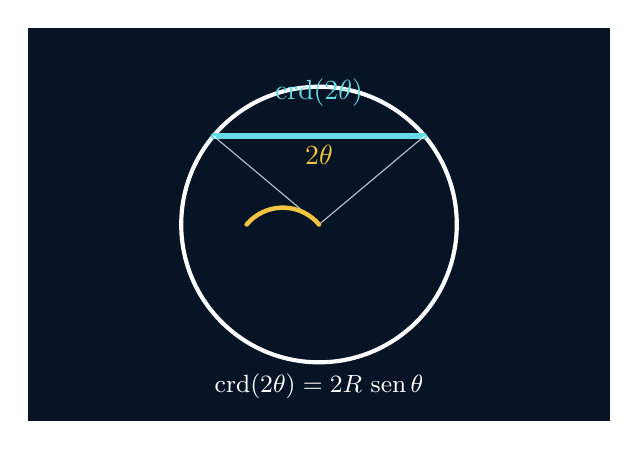
\begin{tikzpicture}[line cap=round,line join=round]
\fill[nostranavy] (-3.7,-2.5) rectangle (3.7,2.5);
\draw[white,line width=1.5pt] (0,0) circle (1.75);
\coordinate (A) at (140:1.75);\coordinate (B) at (40:1.75);
\draw[nostracyan,line width=2pt] (A)--(B);
\draw[white,opacity=.75] (0,0)--(A) (0,0)--(B);
\draw[nostragold,line width=1.6pt] (0,0) arc[start angle=40,end angle=140,radius=.60];
\node[nostragold,font=\bfseries] at (0,.88) {$2\theta$};
\node[nostracyan,font=\bfseries] at (0,1.67) {$\operatorname{crd}(2\theta)$};
\node[white,font=\bfseries\small] at (0,-2.05) {$\operatorname{crd}(2\theta)=2R\,\sen\theta$};
\end{tikzpicture}
\end{document}
